\chapter{Instrukcja użytkownika}

\section{Opis działania menu tablicy}

\subsubsection*{Włączanie}
Po włączeniu ekran inicjuje liczniki, timery, zegar czasu rzeczywistego i~inne. Jednym z~inicjowanych elementów jest obsługa karty pamięci. Ta inicjalizacja często kończy się niepowodzeniem, ekran ją powtarza, aż zakończy się sukcesem. Można anulować ten proces przez naciśnięcie i~przytrzymanie przycisku. Należy tak zrobić przy uruchamianiu ekranu bez karty pamięci. Gdy wszystkie elementy zostaną zainicjowane, jest wyświetlany napis powitalny ,,ekranLED''. 

\subsubsection*{Menu}
W menu jest 5 opcji: ,,zegar'', ,,zegar i~data'', ,,otwórz plik'', ,,ustaw zegar'' i~,,transfer USB''. Zazwyczaj działanie przycisków jest opisane na ekranie. Czasami, gdy jest opisany tylko przycisk A~jako ,,wybierz'', przycisk B oznacza przejście do następnej opcji. Tak jest w~menu i~przy wybieraniu plików.

\begin{figure}[htb]
	\begin{center}
		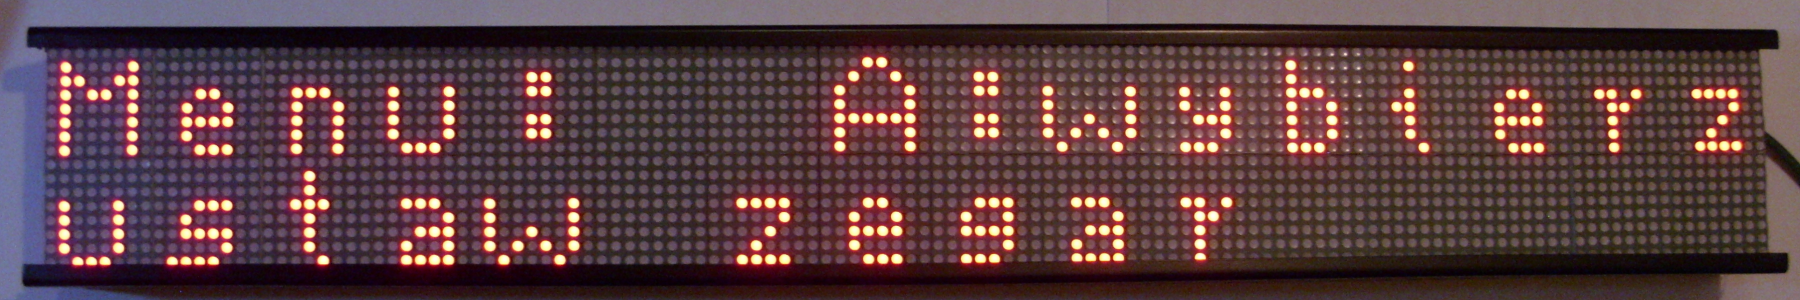
\includegraphics[width=300pt]{figures/screenmenu.png}
	\end{center}
	\caption{Główne menu urządzenia.}
\end{figure}

\subsubsection*{Zegar}
Pierwsze dwie opcje pozwalają wykorzystać ekran bez plików z~animacjami, wyświetlając albo zegar dużo czcionką, albo zegar i~datę małą. Wciśnięcie dowolnego przycisku powoduje wyjście do menu.

\begin{figure}[htb]
	\begin{center}
		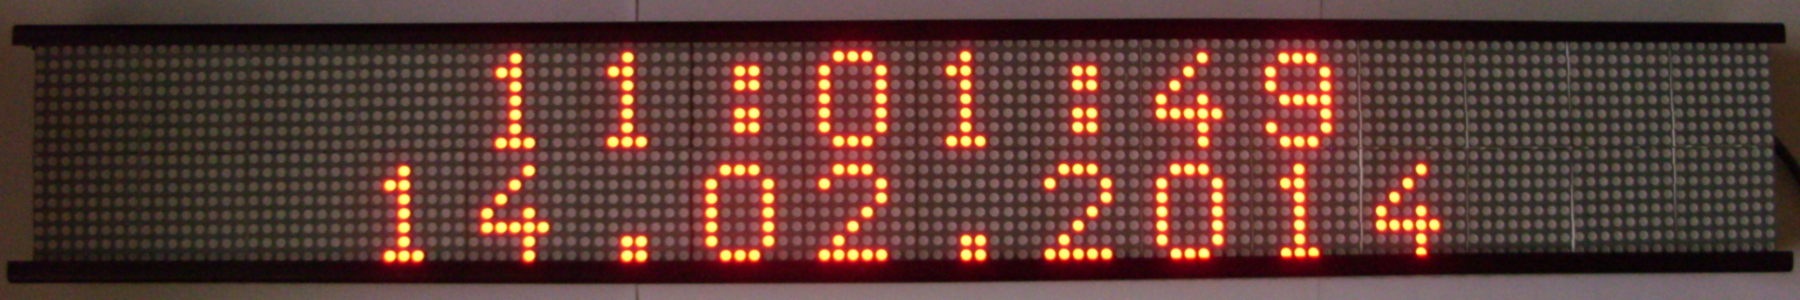
\includegraphics[width=300pt]{figures/zegaridata.png}
	\end{center}
	\caption{Wyświetlanie zagara i daty.}
\end{figure}

\subsubsection*{Otwieranie plików}
Pliki z~animacjami znajdują się na karcie w~folderze /LEDBOARD.~Po wybraniu tego folderu mikrokontroler przelicza znajdujące się tam pliki o~właściwych rozszerzeniach (.m2f i~.mxf). Informacja że nie ma plików (,,0 Plików'') oraz że plik jest pusty (,,Pusty''), zazwyczaj sygnalizują, że karta pamięci nie jest dostępna. Przycisk B przechodzi między plikami, przycisk A~wybiera. Po przejściu przez wszystkie pliki, przed powrotem na początek jest możliwość wyjścia do menu bez otwierania żadnego pliku.

\begin{figure}[htb]
	\begin{center}
		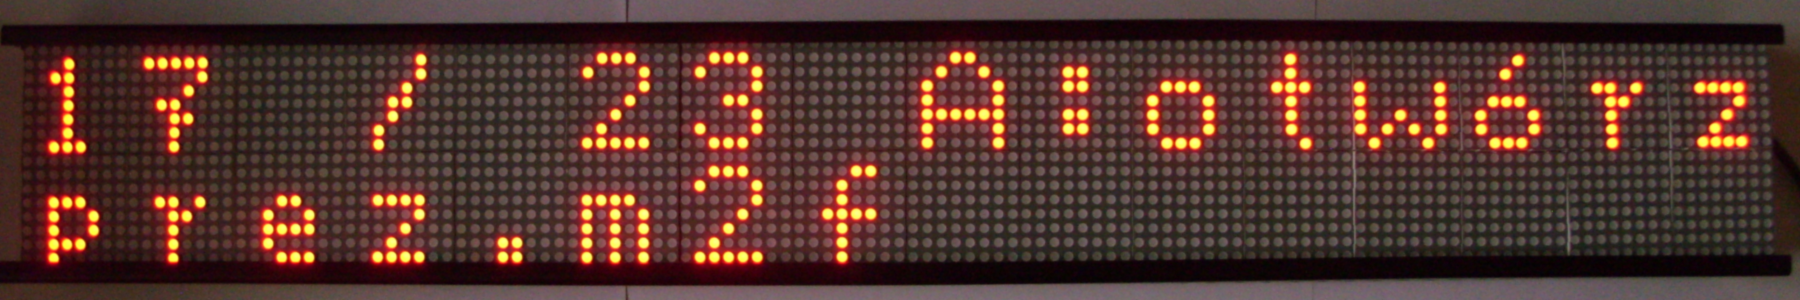
\includegraphics[width=300pt]{figures/wybierzplik.png}
	\end{center}
	\caption{Menu wyboru plików.}
\end{figure}

Gdy zostanie otwarty plik MXF, poprzez naciśnięcie przycisku A~możliwa jest zmiana prędkości przesuwania tekstu. Są dostępne 3 prędkości, przełączane cyklicznie: podstawowa, szybsza, i~najszybsza. Naciśnięcie przycisku B spowoduje powrót do menu. Urządzenie sprawdza stan przycisków tylko gdy właśnie pojawia się kolejna litera, więc aby uzyskać zamierzony efekt, należy przytrzymać przycisk, do momentu zatrzymania tekstu. Puszczenie go wykona zamierzoną akcję.

W trybie wyświetlania pliku M2F, zazwyczaj wciśnięcie dowolnego przycisku powoduje powrót do menu. Inaczej jest gdy wykonywana jest instrukcja czekania na wciśnięcie przycisku. Wtedy naciśnięcie dowolnego przycisku powoduje kontynuację wyświetlania animacji, przejście do kolejnych instrukcji.

\begin{figure}[htb]
	\begin{center}
		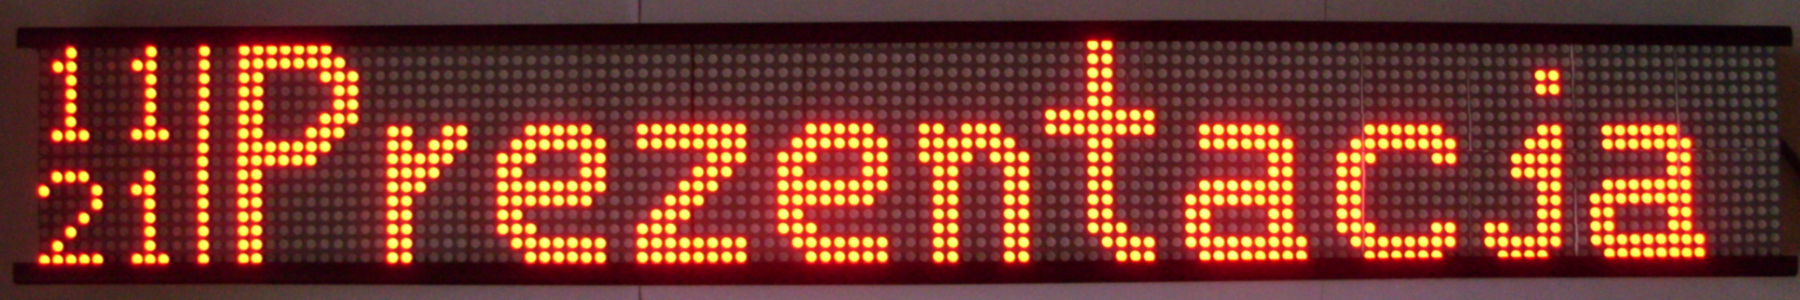
\includegraphics[width=300pt]{figures/prezentacja.png}
	\end{center}
	\caption{Otwarty przykładowy plik z animacją.}
\end{figure}

\subsubsection*{Ustawianie zegara}
Przy ustawianiu zegara najpierw podaje się liczbę godzin, później liczbę minut, po czym albo się zatwierdza wpisany czas, albo wraca do ustawiania godzin. Ustawiony czas jest z~wyzerowanymi sekundami. Napis \texttt{++} oznacza zwiększanie wartości.

Następnie ustawia się datę, w~kolejności rok, miesiąc, dzień.~Taka kolejność jest wymagana, żeby można było określić ile dni ma dany miesiąc w~danym roku. Rok można wybrać z~przedziału od 2000 do 2399, ze względu na to, że układ lat przestępnych ma cykl o~długości 400 lat.

\begin{figure}[htb]
	\begin{center}
		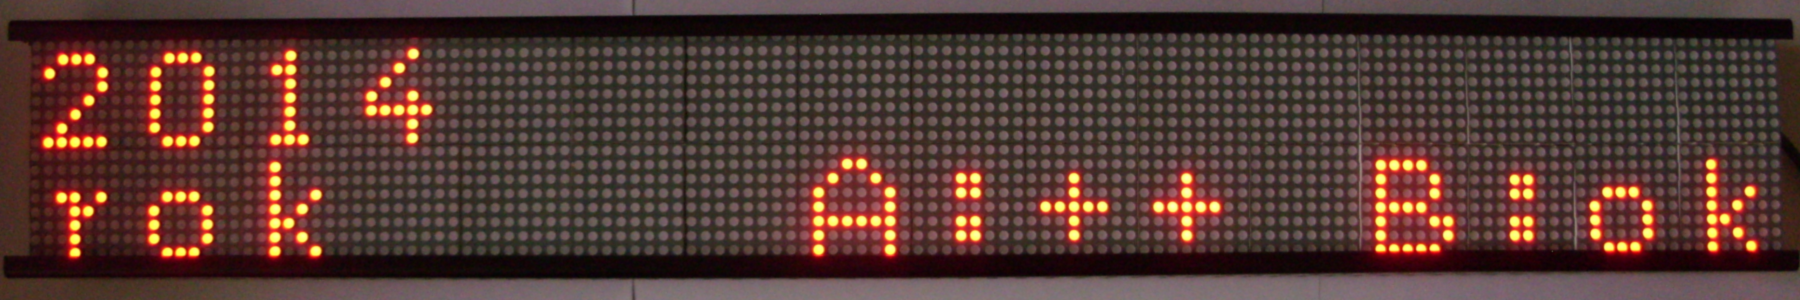
\includegraphics[width=300pt]{figures/ustawzegar.png}
	\end{center}
	\caption{Ustawianie zegara.}
\end{figure}

\subsubsection*{Tryb transferu USB}
W tym trybie można wgrywać pliki na kartę pamięci. Przy włączaniu tego trybu jest inicjowane złącze USB, a~przy wyjściu jest wyłączane. Obok napisu ,,USB'' znajduje się prosta animacja z~przesuwającym się paskiem. Spowolnienie tej animacji oznacza, że odbywa się transmisja. Dowolny przycisk powoduje wyjście z~tego trybu.

\begin{figure}[htb]
	\begin{center}
		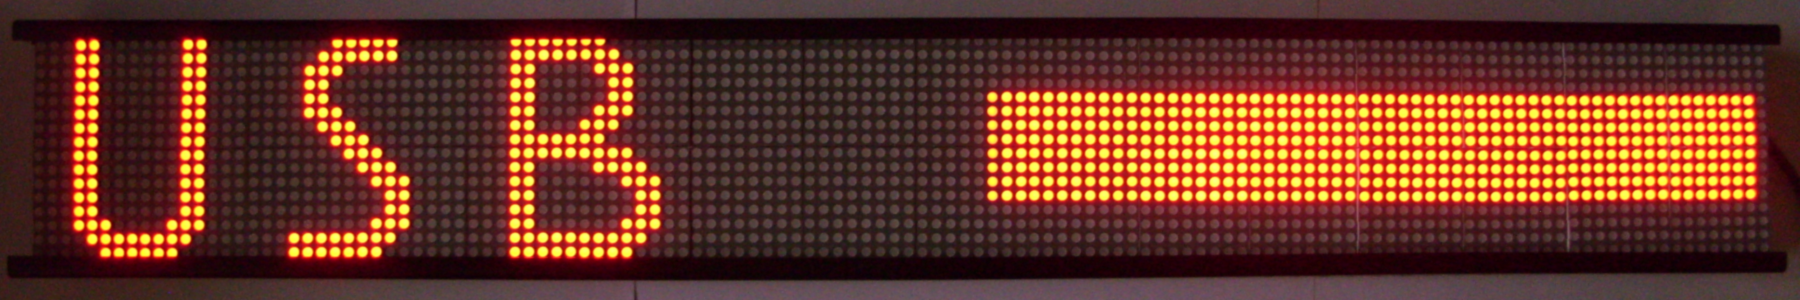
\includegraphics[width=300pt]{figures/trybusb.png}
	\end{center}
	\caption{Ekran trybu transferu USB.}
\end{figure}

\section{Opis tworzenia animacji}

\begin{figure}[htb]
	\begin{center}
		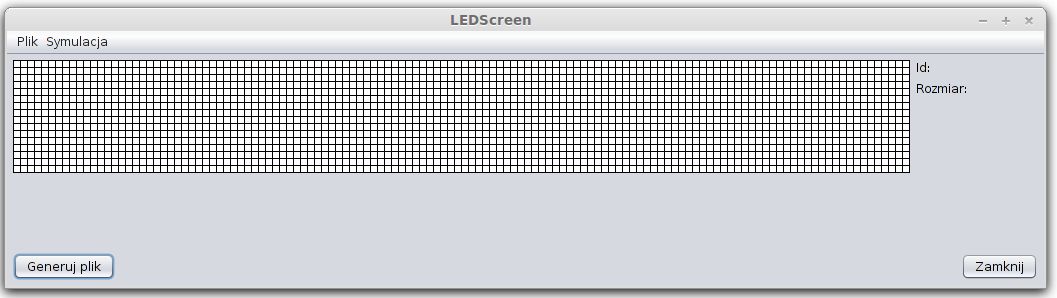
\includegraphics[width=\textwidth]{figures/gui.png}
	\end{center}
	\caption{Główne okno programu użytkownika.}
	\label{mainWindow}
\end{figure}

Główny ekran aplikacji użytkownika przedstawiono na rys. \ref{mainWindow}.  Aby utworzyć obszar (\textit{obszar} --- patrz \ref{slownik}), należy umieścić kursor myszy na powierzchni ekranu tablicy (\textit{ekran} --- patrz \ref{slownik}), wdusić i~przeciągnąć go w~prawo i~w~dół aż do żądanych wymiarów. Podczas rysowania z~prawej strony głównego okna wypisywane zostaną aktualne wymiary obszaru oraz jego identyfikator. Można je również zobaczyć po narysowaniu najeżdżając na któryś z~nich kursorem myszki (patrz rys. \ref{ani-gui2}).

\begin{figure}[htb]
	\begin{center}
		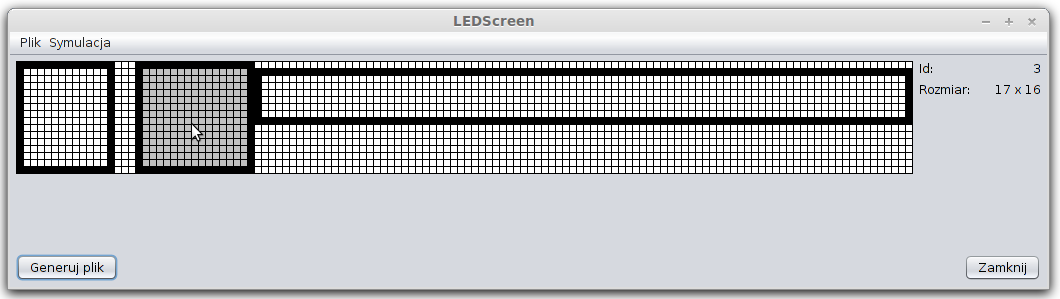
\includegraphics[width=\textwidth]{figures/gui2.png}
	\end{center}
	\caption{Główne okno programu z narysowanymi obszarami.}
	\label{ani-gui2}
\end{figure}

Kliknięcie prawym przyciskiem myszy spowoduje natychmiastowe usunięcie obszaru. Natomiast jeśli użytkownik użyje lewego przycisku, na oknie głównym zostanie wyświetlone okno edycji. Wewnątrz okna edycji użytkownik w~zależności od potrzeb może wybrać dwa tryby klikając na przyciski po lewej stronie: \textit{Tekst} lub \textit{Obraz}. Po zaznaczeniu przycisku uaktywni się żądany tryb edycji obszaru, a~pozostała część się zaciemni.

\begin{figure}[htb]
	\begin{center}
		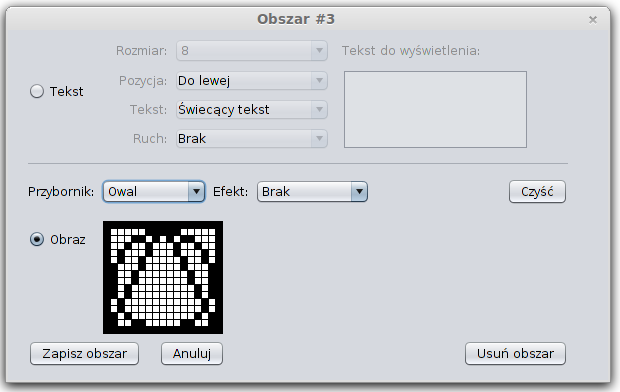
\includegraphics[width=0.8\textwidth]{figures/area.png}
	\end{center}

	\caption{Edycja obszaru w trybie graficznym.}
\end{figure}

W graficznym trybie zaimplementowano przybornik, efekt negatywu oraz przycisk czyszczący ekran. Jeśli negatyw nie jest włączony, ołówek lewym przyciskiem zaznacza piksele czarnym kolorem, natomiast prawym kolorem białym. Przy włączonym efekcie negatywu sytuacja jest odwrotna --- lewy przycisk ,,rysuje'' odznaczając piksele, a~prawy ,,wymazuje''. W~przyborniku znajduje się kilka narzędzi dla użytkownika. Są to: linia, trójkąt, prostokąt i~owal. Rysowanie odbywa się podobnie jak tworzenie obszaru w~głównym oknie, wybierany jest punkt początkowy i~wciśniętym przyciskiem myszy figura jest przeciągana do punktu końcowego. Przy włączonym efekcie negatywu figury ,,rysowane'' są zaznaczając piksele na biało.

\begin{figure}[htb]
	\begin{center}
		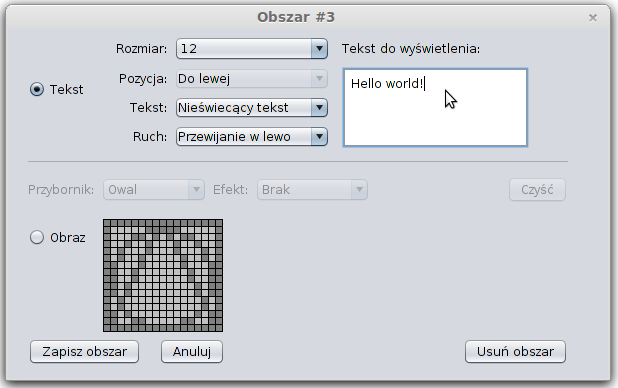
\includegraphics[width=0.8\textwidth]{figures/areaText.png}
	\end{center}
	\caption{Edycja obszaru w trybie tekstowym.}
\end{figure}

W trybie tekstowym kluczowym elementem jest długość tekstu. Jeśli tekst będzie dłuższy niż obszar, natychmiast zniknie większość możliwości ruchu tekstu --- pozostanie przewijanie w~lewo. Oto tekstowe znaki specjalne obsługiwane przez mikroprocesor:

\begin{itemize}
	\item \texttt{$\backslash$G $\backslash$g, $\backslash$M $\backslash$m, $\backslash$S $\backslash$s} --- odpowiednio cyfra dziesiętna i~jedności godzin, cyfra dziesiętna i~jedności minut, cyfra dziesiętna i~jedności sekund aktualnego czasu,
	\item \texttt{$\backslash$D $\backslash$d, $\backslash$K $\backslash$k, $\backslash$R $\backslash$r} --- odpowiednio cyfra dziesiętna i~jedności dnia, cyfra dziesiętna i~jedności miesiąca, cyfra dziesiętna i~jedności roku aktualnej daty,
	\item \texttt{$\backslash$E, $\backslash$o} --- odpowiednio znak euro (\euro) oraz znak stopnia ($^\circ$).
\end{itemize}

Aby zapisać zmiany w~edytowanym obszarze należy uruchomić przycisk \textit{Zapisz obszar}. W~przeciwnym wypadku wprowadzone ustawienia nie zostaną zapisane. Gdy zostały utworzone i~dostosowane wszystkie obszary istnieje możliwość zapisania projektu poprzez wybranie menu \textit{Plik} i~dalej \textit{Zapisz jako}. Zostanie otwarte okno dialogowe i~po wybraniu ścieżki, wpisaniu nazwy pliku i~uruchomieniu przycisku \textit{Zapisz} nastąpi zapis projektu do pliku o~rozszerzeniu \texttt{.mmf} we wskazanym miejscu. Jeśli użytkownik chce, aby animacja została wyświetlana bez przerwy w~pętli, należy przejść do menu \textit{Symulacja} i~zaznaczyć opcję \textit{Animacja w~pętli nieskończonej}. Spowoduje to dodanie na końcu pliku instrukcji dla mikroprocesora, aby wyświetlił animację ponownie.

Jeśli jest potrzeba podglądu animacji --- upewnieniu się, że zaprojektowana animacja zachowuje się tak, jak chciał użytkownik --- można uruchomić menu \textit{Symulacja} i~dalej \textit{Symuluj aktualny projekt}. Pojawi się akno symulacji (patrz rys. \ref{ani-sym}) i~po uruchomieniu symulacji przyciskiem \textit{Start} zostanie odtworzona na ekranie cała zaprojektowana animacja. Jest również możliwość symulowania już wygenerowanych wcześniej plików: menu \textit{Symulacja} i~dalej \textit{Symuluj animaję z~pliku}. Użytkownik zostanie poproszony o~wybranie pliku animacji z~rozszerzeniem \texttt{.m2f}. Po jego wybraniu otworzy się okno z~możliwością odtworzenia symulacji z~pliku.

\begin{figure}[htb]
	\begin{center}
		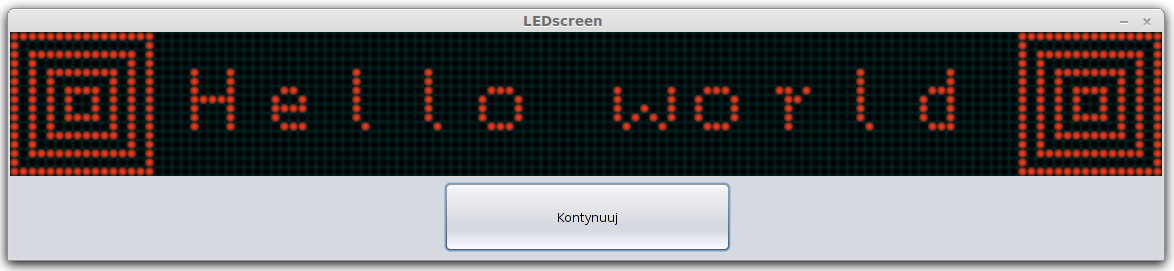
\includegraphics[width=\textwidth]{figures/simulation.png}
	\end{center}
	\caption{Symulacja animacji.}
	\label{ani-sym}
\end{figure}

Aby wygenerować plik animacji należy otworzyć (lub wykonać nowy) projekt i~wcisnąć przycisk \textit{Generuj plik}. Po wybraniu miejsca zapisu i~nazwy pliku program automatycznie wygeneruje plik, który można skopiować do urządzenia (na kartę SD lub poprzez tryb USB), lub zatrzymać na komputerze w~celu późniejszej symulacji. Po skończeniu pracy z~programem należy wcisnąć przycisk \textit{Zamknij}. Jeśli projekt użytkownika nie zostanie wcześniej zapisany przez użytkownika, zostanie utracony.

